\begin{frame}
\titlepage
\end{frame}

\begin{frame}
\frametitle{\centerline{Physics Behind the Simulation: \newline A CS251 Report by Group 22}}
\begin{columns}[T]
\begin{column}{.65\textwidth}
\begin{block}{Simulation}
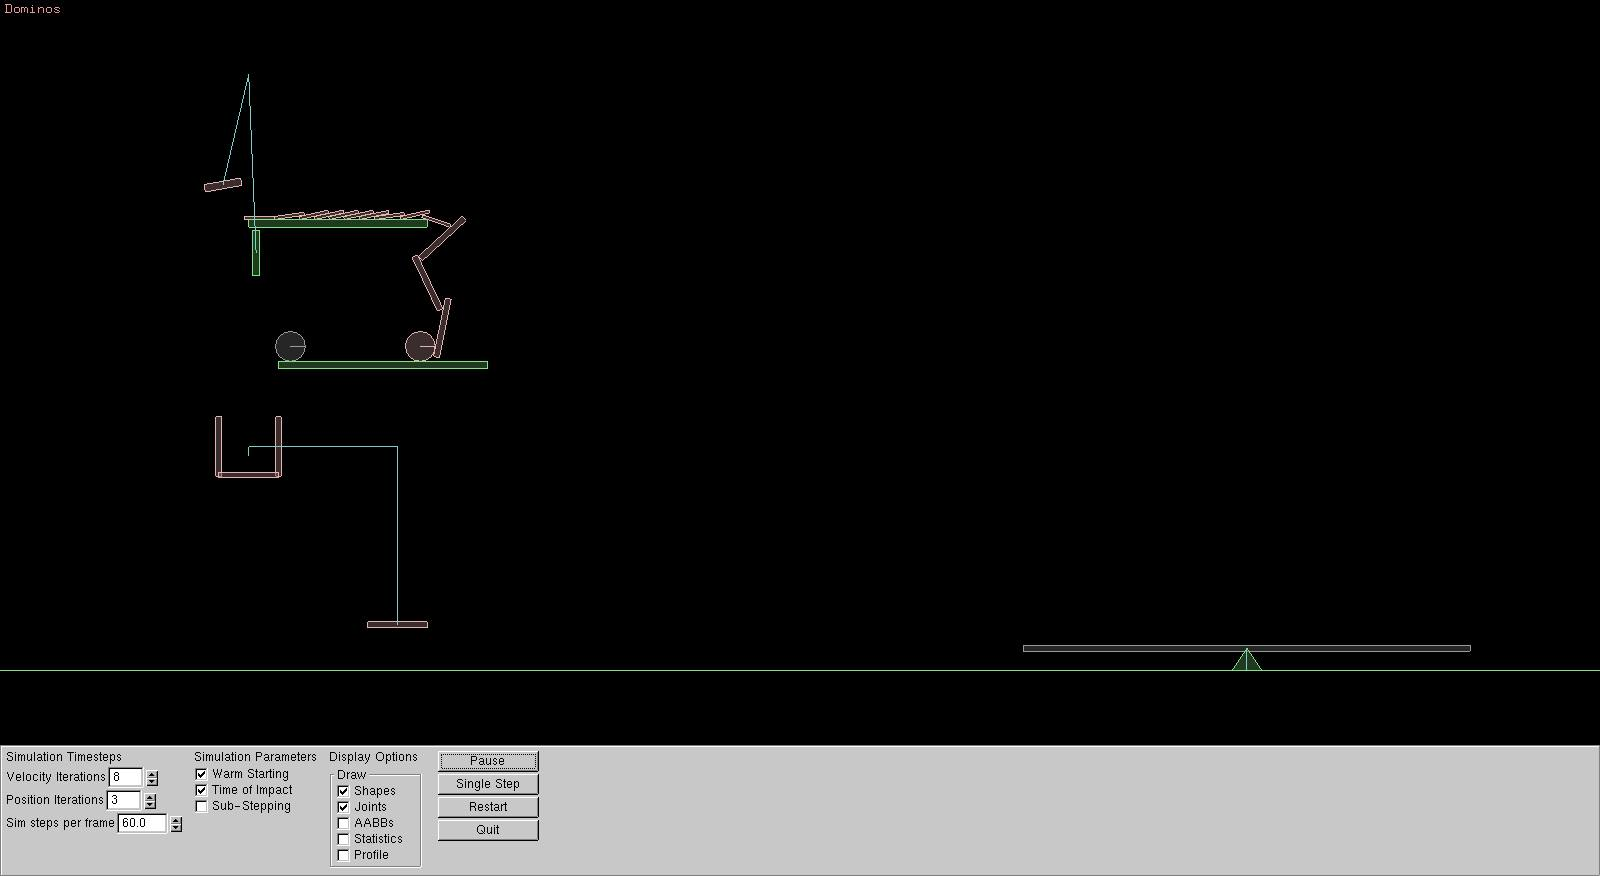
\includegraphics[width=7cm,height=6cm]{box2d.jpg}
\end{block}
\end{column}
\begin{column}{.35\textwidth}
\begin{block}{Contents}
1.Introduction \newline \pause 
2.Body \newline \pause
3.Conclusion \newline \pause
4.References
\end{block}
\end{column}
\end{columns}
\end{frame}

\begin{frame}
\frametitle{\centerline{Introduction}}
This report is created as a part of the documentation of our CS251 project on "Rube Goldberg's Machine" to keep track of the progress of the project over time.
In the coming slides, you will find a detailed description of the progress so far.
Happy Reading!
\end{frame}

\begin{frame}
\frametitle{\centerline{Body}}
\begin{columns}[T]
\begin{column}{.35\textwidth}
\begin{block}{Simulation}
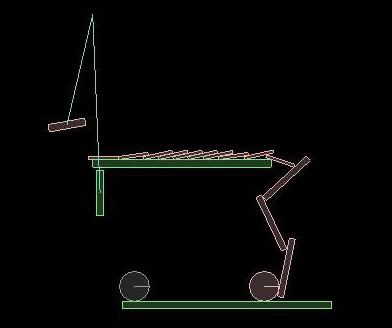
\includegraphics[width=3.8cm,height=3cm]{box2d1.jpg}
\end{block}
\end{column}
\begin{column}{.65\textwidth}
\begin{block}{Contents}
Time period of a compound Pendulum: \newline
$$T=2\pi\sqrt{\frac{I}{mgR}}$$
\fontsize{7pt}{5.2}\selectfont
T (sec) is the time period of a compound pendulum with moment of inertia I ($$kg-m^{2}$$), mass m (kg), acceleration due to gravity g ($$m-sec^{-2}$$), distance from the point of suspension R (m).
\end{block}
\end{column}
\end{columns}
\end{frame}

\begin{frame}
\frametitle{\centerline{Body}}
\begin{columns}[T]
\begin{column}{.35\textwidth}
\begin{block}{Simulation}
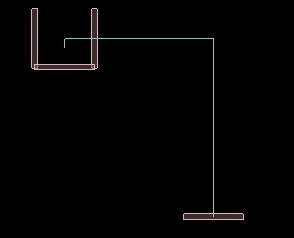
\includegraphics[width=3.8cm,height=3cm]{box2d2.jpg}
\end{block}
\end{column}
\begin{column}{.65\textwidth}
\begin{block}{Contents}
Tension on any rope: \newline
$$T=\frac{2m1m2}{m1+m2}g$$
\fontsize{7pt}{5.2}\selectfont
T (N) is the tension on a rope with mass of the bodies m1 (kg) and m2 (kg) and acceleration due to gravity g ($$m-sec^{-2}$$).
\end{block}
\end{column}
\end{columns}
\end{frame}

\begin{frame}
\frametitle{\centerline{Body}}
\begin{columns}[T]
\begin{column}{.35\textwidth}
\begin{block}{Simulation}

\includegraphics[width=3.8cm,height=3cm]{box2d3.jpg}
\end{block}
\end{column}
\begin{column}{.65\textwidth}
\begin{block}{Contents}
Torque about a hinge: \newline
$$\tau=F.d$$
\fontsize{7pt}{5.2}\selectfont
T (Nm) is the torque about a point when a force F (N) acts at a distance d (m) from the point.
\end{block}
\end{column}
\end{columns}
\end{frame}

\begin{frame}
\frametitle{\centerline{Conclusions}}
This is our idea for the CS251 project. Hope you enjoyed going through the report as much as we are enjoying making it.
In case you are not satisfied, have patience; there are lots of elements to be added yet.
Any other reviews and/or suggetions are most welcome. Looking forward to hearing from you.
\end{frame}

\begin{frame}
\frametitle{\centerline{References}}
\cite{Stack}
\cite{Doxygen}
\cite{Linux}
\bibliography{beamer}
\bibliographystyle{ieeetr}
\end{frame}
